% Page: Smooth means
% sources/book/chapters/06-smooth-means.qmd
% The roughness penalty on that page. A straight line has second derivative
% zero, so as lambda -> infinity the fit is the least-squares line and the
% equivalent degrees of freedom fall to 1. As lambda -> 0 the cubic spline
% interpolates every distinct x. The middle curve is a cubic spline with an
% intermediate second-difference penalty. Schematic points, not the lidar data.
\documentclass[border=6pt]{standalone}
\usepackage[T1]{fontenc}
\usepackage{lmodern}
\usepackage{amsmath,amssymb}
\usepackage{tikz}
\usepackage{pgfplots}
\pgfplotsset{compat=1.18}
\definecolor{ink}{HTML}{1F2430}
\definecolor{statblue}{HTML}{174A7E}
\definecolor{grey}{HTML}{5E6A75}
\pgfplotsset{
  stat/.style={
    scale only axis,
    axis lines=left,
    axis line style={ink, line width=0.6pt},
    tick style={ink, line width=0.45pt},
    tick label style={font=\small, text=ink},
    label style={font=\small, text=ink},
    title style={font=\small, text=ink, align=center},
    legend style={font=\small, draw=none, fill=none, text=ink,
      cells={anchor=west}, inner sep=1.5pt,
      at={(0.98,0.03)}, anchor=south east},
    unbounded coords=jump,
    scaled ticks=false,
  },
}
\begin{document}
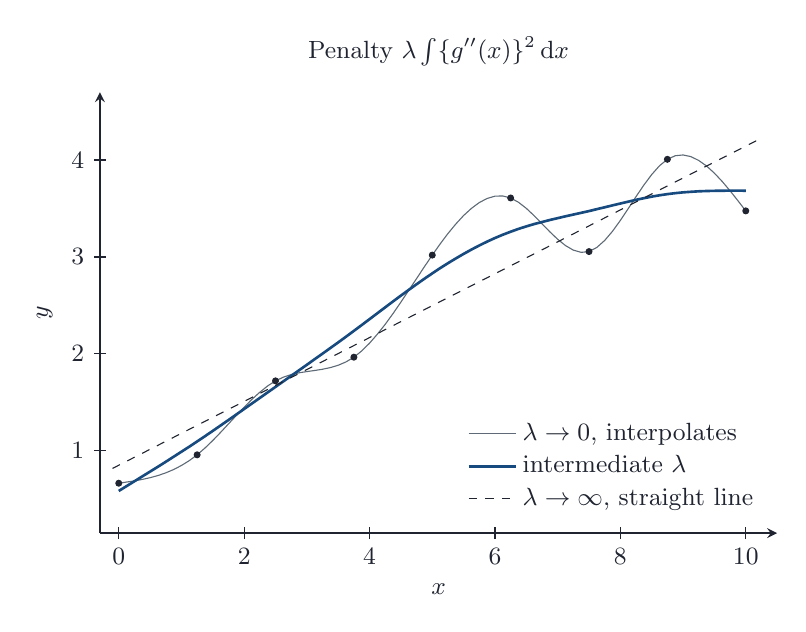
\begin{tikzpicture}
\begin{axis}[
  stat, width=8.6cm, height=5.6cm,
  xmin=-0.3, xmax=10.5, ymin=0.15, ymax=4.7,
  xtick={0,2,4,6,8,10},
  ytick={1,2,3,4},
  xlabel={$x$},
  ylabel={$y$},
  title={Penalty $\lambda\int\{g''(x)\}^{2}\,\mathrm{d}x$},
]
  \addplot[grey, thin] coordinates {
(0.000,0.665) (0.125,0.677) (0.250,0.689) (0.375,0.704)
    (0.500,0.722) (0.625,0.744) (0.750,0.772) (0.875,0.806)
    (1.000,0.848) (1.125,0.898) (1.250,0.958) (1.375,1.028)
    (1.500,1.106) (1.625,1.190) (1.750,1.277) (1.875,1.364)
    (2.000,1.450) (2.125,1.531) (2.250,1.604) (2.375,1.669)
    (2.500,1.721) (2.625,1.759) (2.750,1.786) (2.875,1.804)
    (3.000,1.817) (3.125,1.828) (3.250,1.841) (3.375,1.858)
    (3.500,1.882) (3.625,1.917) (3.750,1.965) (3.875,2.030)
    (4.000,2.110) (4.125,2.203) (4.250,2.305) (4.375,2.416)
    (4.500,2.534) (4.625,2.655) (4.750,2.777) (4.875,2.899)
    (5.000,3.019) (5.125,3.133) (5.250,3.241) (5.375,3.339)
    (5.500,3.427) (5.625,3.501) (5.750,3.561) (5.875,3.603)
    (6.000,3.627) (6.125,3.629) (6.250,3.608) (6.375,3.564)
    (6.500,3.501) (6.625,3.425) (6.750,3.342) (6.875,3.259)
    (7.000,3.182) (7.125,3.117) (7.250,3.070) (7.375,3.047)
    (7.500,3.055) (7.625,3.098) (7.750,3.170) (7.875,3.265)
    (8.000,3.377) (8.125,3.498) (8.250,3.622) (8.375,3.742)
    (8.500,3.850) (8.625,3.941) (8.750,4.007) (8.875,4.044)
    (9.000,4.052) (9.125,4.035) (9.250,3.995) (9.375,3.938)
    (9.500,3.864) (9.625,3.778) (9.750,3.682) (9.875,3.580)
    (10.000,3.475)
  };
  \addlegendentry{{$\lambda\to 0$, interpolates}}
  \addplot[statblue, line width=0.95pt] coordinates {
(0.000,0.585) (0.125,0.635) (0.250,0.685) (0.375,0.735)
    (0.500,0.785) (0.625,0.835) (0.750,0.886) (0.875,0.938)
    (1.000,0.990) (1.125,1.042) (1.250,1.096) (1.375,1.150)
    (1.500,1.205) (1.625,1.261) (1.750,1.317) (1.875,1.374)
    (2.000,1.431) (2.125,1.488) (2.250,1.545) (2.375,1.602)
    (2.500,1.659) (2.625,1.716) (2.750,1.773) (2.875,1.830)
    (3.000,1.887) (3.125,1.945) (3.250,2.002) (3.375,2.060)
    (3.500,2.118) (3.625,2.177) (3.750,2.237) (3.875,2.297)
    (4.000,2.358) (4.125,2.419) (4.250,2.480) (4.375,2.541)
    (4.500,2.601) (4.625,2.660) (4.750,2.718) (4.875,2.775)
    (5.000,2.830) (5.125,2.884) (5.250,2.935) (5.375,2.984)
    (5.500,3.031) (5.625,3.076) (5.750,3.118) (5.875,3.158)
    (6.000,3.195) (6.125,3.229) (6.250,3.260) (6.375,3.289)
    (6.500,3.315) (6.625,3.339) (6.750,3.360) (6.875,3.381)
    (7.000,3.400) (7.125,3.419) (7.250,3.437) (7.375,3.455)
    (7.500,3.473) (7.625,3.493) (7.750,3.512) (7.875,3.532)
    (8.000,3.551) (8.125,3.570) (8.250,3.589) (8.375,3.606)
    (8.500,3.622) (8.625,3.636) (8.750,3.648) (8.875,3.658)
    (9.000,3.666) (9.125,3.672) (9.250,3.677) (9.375,3.680)
    (9.500,3.682) (9.625,3.683) (9.750,3.684) (9.875,3.684)
    (10.000,3.683)
  };
  \addlegendentry{intermediate $\lambda$}
  \addplot[ink, dashed, thin, domain=-0.1:10.2, samples=2] {0.850376+0.329326*x};
  \addlegendentry{{$\lambda\to\infty$, straight line}}
  \addplot[only marks, mark=*, mark size=1.05pt, ink, forget plot] coordinates {
    (0,0.6649) (1.25,0.9579) (2.5,1.7207) (3.75,1.9654) (5,3.0187)
    (6.25,3.6082) (7.5,3.0552) (8.75,4.0072) (10,3.4749)
  };
\end{axis}
\end{tikzpicture}
\end{document}
